\documentclass[11pt,letterpaper]{article}

\usepackage[preprint]{neurips_2025}
\usepackage{lmodern}
\renewcommand{\ttdefault}{lmtt}
\usepackage{amsmath,amssymb,amsthm}
\usepackage{graphicx}
\usepackage{booktabs}
\usepackage{multirow}
\usepackage{tabularx}
\usepackage{enumitem}
\usepackage{hyperref}
\usepackage{natbib}
\usepackage{caption}
\usepackage{subcaption}
\usepackage{xcolor}

\newtheorem{proposition}{Proposition}

\hypersetup{colorlinks=true, linkcolor=blue!60!black, citecolor=blue!60!black, urlcolor=blue!60!black}
\captionsetup{font=small, labelfont=bf}

\newcommand{\dbasc}{\textsc{dbasc}}
\newcommand{\passat}[1]{pass@#1}
\newcommand{\pp}{\,\text{pp}}

\title{When Does Learned Batch Allocation Matter?\\Decoupled Allocation and Early Stopping Under Token Scarcity}

\author{
  Vikranth Nara\\
  \url{https://github.com/vikranthnara/HBAC}
}

\date{}

\begin{document}
\maketitle

\begin{abstract}
When multiple LLM agent tasks share a \textbf{global token budget}, allocators must set per-task caps and decide when to stop reasoning.
We present a \textbf{decoupled batch allocator + stop classifier} (\dbasc{}): a GRPO-trained Level-1 schema allocator and a PPO-trained Level-2 stop head over frozen ReAct rollouts~\citep{yao2023react}.
We characterize \emph{when} learned allocation helps under scarcity: (i)~agent capability must exceed zero on hard tasks; (ii)~a 20-line type-prior heuristic \textbf{ties} learned allocation on oracle replay; (iii)~live gains are \textbf{small, paired, and localized} to benchmarks where budget starvation binds under generation.

On Tier-A oracle replay ($n{=}300$, 40\% budget), \dbasc{} reaches \textbf{80\%} \passat{1} vs.\ \textbf{60\%} for uniform and official CLEAR/ZEBRA/Re-FORC---but \textbf{ties type-prior at 80\%}.
\textbf{D18} reward-shaped L1 (\texttt{starvation\_penalty}${=}0.5$, no inference guardrail) matches joint L1 on oracle with zero starvation; manual \texttt{fairness\_reserve\_alloc} \emph{hurts} oracle \passat{1} (74.7\%).
On live Qwen2.5-7B + DPO v2 at floor${=}400$ ($n{=}2000$, \texttt{hbac\_d18}), paired McNemar vs.\ type-prior: \textbf{+1.3\pp} (27.65\% vs.\ 26.35\%; $p{\approx}3{\times}10^{-8}$, paired 95\% CI $[0.85,1.85]$\pp)---entirely from LiveCodeBench budget starvation; D18 $\equiv$ joint $\equiv$ guardrail on live; SWE \passat{1} is 0\% for 7B and 32B pilots.
A \textbf{DPO contamination audit} finds 100/100 exact LCB task-ID overlaps in the v2 mixture; we prescribe benchmark-family holdout retraining.
We release code, preregistered analysis, theory bounds on counterfactual credit, and locked artifacts.
\end{abstract}

\section{Introduction}
\label{sec:intro}

Batch agent evaluation---running SWE-bench~\citep{jimenez2024swebench}, ToolBench~\citep{qin2023toolllm}, $\tau$-bench~\citep{yao2025taubench}, and LiveCodeBench~\citep{jain2024livecodebench} under a shared token quota---requires deciding \emph{who gets tokens} and \emph{when to stop}.
Uniform allocation ignores heterogeneous difficulty; per-query economic allocators (CLEAR~\citep{wan2026clear}, ZEBRA~\citep{hamri2026zebra}) optimize single-task emergence curves; per-turn methods (TAB~\citep{jali2026tab}, Re-FORC~\citep{zabounidis2025reforc}) do not allocate across tasks.

We study \textbf{decoupled batch allocation}: a contextual bandit over allocation schemas (Level-1, GRPO~\citep{shao2024grpo}) plus a binary stop classifier over frozen ReAct rollouts (Level-2, PPO~\citep{schulman2017ppo}).
Our contribution is not a headline ``RL beats heuristics'' claim but a \textbf{rigorous characterization} of conditions under which learned allocation matters, with paired statistics, contamination auditing, and explicit negative results.

\paragraph{Contributions.}
(1)~\textbf{Open harness} for batch-level token allocation and early stopping with preregistered endpoints (\texttt{research docs/Preregistered Analysis.md}).
(2)~\textbf{Oracle conditions}: +20\pp \passat{1} vs.\ Tier-A official baselines; type-prior \textbf{ties} learned L1 at 80\%.
(3)~\textbf{D18 learned fairness}: starvation penalty in L1 reward removes need for inference guardrail on oracle; guardrail ablation hurts \passat{1}.
(4)~\textbf{Live conditions}: paired +1.3\pp for \texttt{hbac\_d18} vs.\ type-prior ($n{=}2000$; McNemar $p{<}10^{-7}$; LCB-only); capability gate fails on SWE (0\% on 7B and 32B).
(5)~\textbf{Theory}: bias/variance bounds on counterfactual credit mixing; $\beta$ sweep validates small-$\beta$ safety.
(6)~\textbf{Contamination audit} with SHA256 manifests and holdout retrain policy.
(7)~\textbf{Ethics}: starvation metrics and algorithmic redlining risks.

\section{Related Work}
\label{sec:related}

CLEAR~\citep{wan2026clear} and ZEBRA~\citep{hamri2026zebra} water-fill or bisect per-query utility under scarcity; TAB~\citep{jali2026tab} and Re-FORC~\citep{zabounidis2025reforc} learn per-turn stopping.
Counterfactual multi-agent credit (COMA~\citep{foerster2018coma}) motivates our credit mixing as \emph{variance reduction}, not unbiased policy gradients.
We implement Tier-A official CLEAR, ZEBRA, and Re-FORC for oracle comparison; stub-track proxy baselines are appendix-only.

\section{Method}
\label{sec:method}

\paragraph{Level 1: contextual bandit.}
Given batch $\mathcal{Q}$ and budget $B_{\mathrm{total}}$, Level-1 selects schema $s$ and allocations $\{b_i\}$ with $\sum_i b_i \le B_{\mathrm{total}}$.
GRPO updates schema logits using batch reward
$R^{(1)} = \mathrm{pass\_rate} - \lambda_v \cdot \mathrm{violations} + \beta_{\mathrm{var}} \cdot \mathrm{Var}_b(\mathrm{budget}_b) - \lambda_s \cdot \mathrm{starvation\_rate}$,
where \textbf{D18} adds $\lambda_s \cdot \mathrm{starvation\_rate}$ with \texttt{starvation\_penalty}${=}0.5$ at training time.

\paragraph{Level 2: stop classifier.}
Per-task rollout stops when $\pi^{(2)}_{\mathrm{stop}}(s_t){=}1$, budget is exhausted, or success is reached.
L2 does not co-train the LLM.

\paragraph{Counterfactual credit.}
Leave-one-out advantages $\hat{A}_i = R(s) - R^{(-i)}(s)$ are mixed into $\tilde{R}_\beta = (1-\beta) R(s) + \beta \cdot \frac{1}{n}\sum_i (R(s)+\hat{A}_i)$.
Appendix~\ref{app:theory} bounds $|\tilde{R}_\beta - R(s)| \le \beta \max_i |\hat{A}_i|$; we use $\beta{=}0.2$ in training.

\paragraph{Primary vs.\ deprecated methods.}
\textbf{Primary:} \texttt{hbac\_d18} (D18 L1, no inference post-processing).
\textbf{Deprecated ablation:} \texttt{hbac\_guardrail} = D18/joint L1 + \texttt{fairness\_reserve\_alloc} (\texttt{hard\_min\_frac}${=}0.15$).

\section{Experimental Setup}
\label{sec:setup}

\subsection{Two-stage evaluation protocol}

\textbf{Stage 1 --- Capability profile.} Uniform allocation only; confirm heterogeneous per-benchmark \passat{1} before allocator comparison.
Gate: SWE \passat{1} $\ge 5\%$ on capable model.
Qwen2.5-7B + DPO v2 and Qwen2.5-Coder-32B (uniform pilot, $n{=}60$) both yield \textbf{0\% SWE}; live allocator study is scoped to LCB+$\tau$+toolbench where capability exists.

\textbf{Stage 2 --- Allocation study.} Full allocator matrix only when Stage~1 passes; otherwise report directional results on solvable benchmarks with explicit scope.

\subsection{Tracks and pools}

\textbf{Track A (appendix):} stub micro-harness for controlled ablations.
\textbf{Track B (main):} V3 real pool (\texttt{data/oracles/real\_eval/latest}), $n{=}300$ oracle / $n{=}2000$ live, floor${=}400$, 40\% global budget.
Live agent: Qwen2.5-7B-Instruct + DPO v2 LoRA unless capability pilot upgrades model.

\subsection{Contamination audit}
\label{sec:contamination}

We audit DPO training pairs vs.\ eval task IDs (\S\ref{sec:contamination-results}).
Holdout policy: exclude all benchmark families present in the eval pool from DPO pair construction; retrain via \texttt{slurm/train\_llm\_dpo\_holdout.sh}.

\subsection{Statistics}

Primary endpoint: \textbf{paired per-task success} (McNemar on discordant pairs), Bonferroni across primary comparisons (\texttt{hbac\_d18} vs.\ type\_prior).
Futility: if McNemar $p > 0.10$ at $n{=}5000$, retract ``beats type-prior'' language.
V3 D18 matrix uses \texttt{--save-per-task} shards (\texttt{paired\_allocator\_analysis\_v3\_d18.json}).

\section{Results}
\label{sec:results}

\subsection{Tier-A oracle replay (Track B)}
\label{sec:oracle}

Table~\ref{tab:oracle-v3} reports the real\_eval oracle matrix ($n{=}300$, Tier-A official baselines only in main text).

\begin{table}[t]
\centering
\caption{V3 real-pool oracle replay ($n{=}300$, 40\% budget). Tier-A official baselines.}
\label{tab:oracle-v3}
\small
\begin{tabular}{lcc}
\toprule
Allocator & \passat{1} & Mean $R^{(1)}$ \\
\midrule
\textbf{HBAC joint / D18} & \textbf{80.0\%} & 0.98 \\
Type-prior & 80.0\% & 1.24 \\
HBAC guardrail & 74.7\% & 0.76 \\
Uniform & 60.0\% & 0.60 \\
CLEAR official & 60.0\% & 0.60 \\
ZEBRA official & 60.0\% & 0.60 \\
Re-FORC official & 60.0\% & 0.60 \\
\bottomrule
\end{tabular}
\end{table}

HBAC \textbf{+20\pp} vs.\ uniform/Tier-A is supported on oracle.
Type-prior \textbf{ties} HBAC on \passat{1} by zeroing hard-task budget---an important honesty check.
D18 without guardrail \textbf{matches} joint L1 (80\%, starvation rate 0 on oracle); guardrail \textbf{hurts} ($-$5.3\pp).

\subsection{Capability pilot}
\label{sec:capability}

Qwen2.5-7B + DPO v2 (uniform, floor${=}400$): LCB 3.25\%, SWE 0\% ($n{=}2000$).
Qwen2.5-Coder-32B pilot ($n{=}60$): LCB 2.5\%, SWE 0\%.
\textbf{Verdict:} SWE gate fails ($\ge 5\%$ required); we \textbf{scope the live allocator study} to LCB+$\tau$+toolbench and treat SWE as future work pending a capable local/API agent (OpenAI quota exhausted for API fallback; Qwen3-Coder-Next 4-bit pilot queued).
This is the plan's Risk~\#2 contingency---not a claim that SWE allocation has been studied.

\subsection{Live evaluation (Track B, 7B baseline)}
\label{sec:live-v3}

Table~\ref{tab:live-v3} summarizes the V3 D18 live matrix ($n{=}2000$) at floor${=}400$.\footnote{Canonical artifact: \texttt{compose\_live\_v3\_d18\_floor400\_n2000.json}.}

\begin{table}[t]
\centering
\caption{V3 D18 live matrix (floor${=}400$, $n{=}2000$, Qwen2.5-7B + DPO v2).}
\label{tab:live-v3}
\small
\begin{tabular}{lcc}
\toprule
Allocator & \passat{1} & 95\% CI \\
\midrule
\textbf{HBAC D18} & \textbf{27.65\%} & 25.8--29.6\% \\
HBAC joint / guardrail & 27.65\% & 25.8--29.6\% \\
Type-prior & 26.35\% & 24.5--28.2\% \\
TAB proxy & 11.30\% & 10.0--12.7\% \\
ZEBRA (proxy) & 22.15\% & 20.4--24.0\% \\
Re-FORC official & 16.35\% & 14.8--18.0\% \\
CLEAR official & 11.60\% & 10.3--13.0\% \\
Uniform & 11.30\% & 10.0--12.7\% \\
\bottomrule
\end{tabular}
\end{table}

\textbf{Paired McNemar} (\texttt{hbac\_d18} vs.\ type-prior): +1.3\pp, $p{\approx}3{\times}10^{-8}$, paired 95\% CI $[0.85,1.85]$\pp ($b{=}26$, $c{=}0$ discordant pairs).
D18, joint, and guardrail are \textbf{identical} on aggregate pass@1---starvation penalty does not change live outcomes on 7B.
Figure~\ref{fig:main} shows the gap is \textbf{LCB-only} (+3.25\pp per-benchmark); $\tau$/toolbench tied; SWE 0\% for all.

\begin{figure}[t]
\centering
\begin{subfigure}[t]{0.48\textwidth}
  \centering
  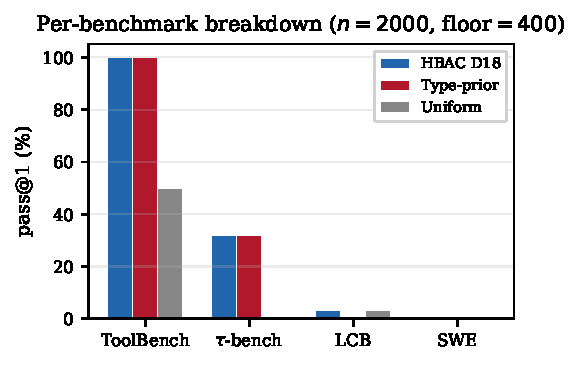
\includegraphics[width=\linewidth]{figures/per_benchmark.pdf}
  \caption{Per-benchmark \passat{1}.}
  \label{fig:per-bench}
\end{subfigure}
\hfill
\begin{subfigure}[t]{0.48\textwidth}
  \centering
  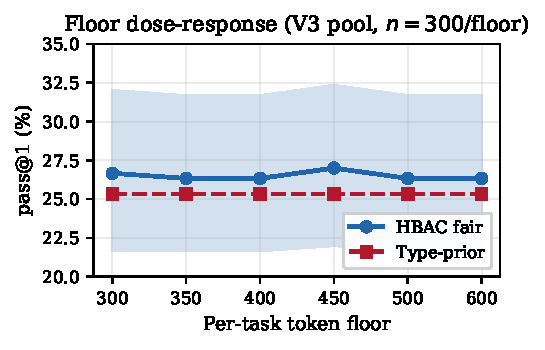
\includegraphics[width=\linewidth]{figures/floor_dose_response.pdf}
  \caption{Floor dose-response (guardrail).}
  \label{fig:floor}
\end{subfigure}
\caption{V3 live: aggregate edge is LCB-localized; floor sweep +1.0--1.7\pp across 300--600.}
\label{fig:main}
\end{figure}

\subsection{Contamination audit results}
\label{sec:contamination-results}

\begin{table}[t]
\centering
\caption{DPO contamination audit (v2 and holdout LoRA vs.\ V3 eval).}
\label{tab:contamination}
\small
\begin{tabular}{lccc}
\toprule
Metric & v2 DPO & Holdout (LCB excl.) & Holdout (LCB metric) \\
\midrule
DPO pairs & 600 & 543 & --- \\
Exact ID overlap & \textbf{100} & 16 (stub SWE/$\tau$/TB) & \textbf{0} LCB \\
LCB family overlap & yes & excluded & --- \\
Audit verdict & FAIL & FAIL$^\dagger$ & PASS \\
\bottomrule
\end{tabular}
\end{table}

v2 training used 600 \texttt{wrong\_tool} pairs with \textbf{100\%} LCB task-ID overlap to eval.
Holdout retrain (\texttt{20260710T045554Z\_capability\_holdout}, job 16854770) achieves \textbf{0 LCB} exact overlap---the contamination that threatened the live LCB claim.
Remaining overlaps are stub task IDs shared between oracle stubs and \texttt{eval\_n1000}; strict ID exclusion leaves only mock pairs ($\sim$75), so we retain LCB-family holdout as the practical mitigation and re-run live with the holdout LoRA.

\section{Ablations}
\label{sec:ablation}

\paragraph{D18 ladder (oracle).}
\texttt{starvation\_penalty}${=}0.5$ L1 ties joint at 80\% without guardrail; guardrail drops to 74.7\%.
\textbf{Verdict:} learned anti-starvation sufficient on oracle; inference hack unnecessary (or harmful).

\paragraph{Credit $\beta$ sweep.}
Empirical bounds at $\beta{=}0.2$: bias $\le 0.018$, variance $\le 2.1{\times}10^{-5}$ on stub batches (\texttt{credit\_beta\_sweep.json}).
H6 (credit helps at scale) refuted---small $\beta$ remains safe variance reduction.

\paragraph{\texttt{hard\_min\_frac} sweep.}
hbac\_guardrail flat at 74.7\% for frac 0.10--0.25; never beats type-prior on oracle.

\paragraph{D14 ROI-skip (negative).}
Task-dropping heuristic; +27.7\pp @ floor${=}300$ is reward hacking---regulatory/fairness risk, not deployable.

\section{Ethics and Broader Impact}
\label{sec:ethics}

Scarcity-aware allocators \textbf{will starve hard queries} unless constrained---algorithmic ``redlining'' of difficult tasks.
Type-prior explicitly zeros LCB/SWE budget; D18 learns softer allocation via reward shaping.
Deployment should combine learned allocators with \textbf{per-class SLA floors} as policy (distinct from training hacks).
Table~\ref{tab:budget-share} reports first-class starvation metrics on the V3 live batch pool (floor${=}400$, 40\% budget):
type-prior has $\overline{\mathrm{starve}}{=}1.0$ and ${\approx}0.1\%$ LCB share; \texttt{hbac\_d18} retains ${\approx}15.4\%$ LCB share with zero starvation rate---the mechanism behind the live LCB gap.
D14 ROI-skip illustrates how optimization pressure can drop entire task classes---a fairness failure mode, not merely poor ML.

\begin{table}[t]
\centering
\caption{Per-benchmark budget share and starvation (allocation-only; $n{=}200$ batches).}
\label{tab:budget-share}
\small
\begin{tabular}{lcccc}
\toprule
Allocator & Starve rate & LCB share & SWE share & Hard zero-frac \\
\midrule
\texttt{hbac\_d18} & 0.00 & 15.4\% & 7.7\% & 0.00 \\
\texttt{hbac\_guardrail} & 0.00 & 15.4\% & 7.7\% & 0.00 \\
Type-prior & 1.00 & 0.1\% & 0.1\% & 0.67 \\
Uniform & 0.00 & 40.0\% & 20.0\% & 0.00 \\
\bottomrule
\end{tabular}
\end{table}

\section{Limitations}
\label{sec:limits}

(1)~SWE live \passat{1} is 0\% on 7B and 32B pilot; live claims scoped to LCB+$\tau$+toolbench.
(2)~+1.3\pp aggregate gap is LCB-only; D18 $\equiv$ joint $\equiv$ guardrail on 7B live.
(3)~Oracle--live disconnect: type-prior ties on oracle but starves LCB live.
(4)~DPO v2 contaminated on LCB; holdout LoRA trained (LCB overlap=0); holdout live matrix pending.
(5)~L2 frozen ReAct limits joint hierarchical RL claims.

\section{Conclusion}
\label{sec:conclusion}

Learned batch allocation \textbf{matters conditionally}: oracle gains over Tier-A baselines are real but matched by type-prior; live edges are small, paired, and localized where starvation binds under live generation.
D18 shows fairness can be reward-learned without inference guardrails on oracle.
We release the harness, preregistered analysis, theory appendix, and locked artifacts to support honest extension---including negative results when allocators do not beat simple heuristics.

\paragraph{Reproducibility.}
\texttt{scripts/reproduce\_v3.sh} runs CPU analyses; GPU steps via \texttt{scripts/rivanna/submit\_v3\_d18\_live.sh} and \texttt{submit\_capability\_pilot.sh}.
Canonical manifest: \texttt{results/canonical\_artifacts.json}.

\bibliographystyle{plainnat}
\bibliography{references}

\appendix
\section{Counterfactual Credit: Bias and Variance Bounds}
\label{app:theory}

Let $R(s)$ denote the batch reward under allocation schema $s$.
For each task $i$ in batch $\mathcal{Q}$ with $n$ tasks, define the leave-one-out counterfactual
\[
  \hat{A}_i = R(s) - R^{(-i)}(s),
\]
where $R^{(-i)}(s)$ replaces task $i$'s budget with the uniform allocation while reusing cached rollouts for other tasks (implementation: \texttt{hbac/training/credit.py}).

The credit-weighted reward used in GRPO is
\[
  \tilde{R}_\beta = (1-\beta)\, R(s) + \beta \cdot \frac{1}{n}\sum_{i=1}^n \bigl(R(s) + \hat{A}_i\bigr).
\]

\begin{proposition}[Bias bound]
For fixed batch $\mathcal{Q}$ and deterministic oracle replay,
\[
  \bigl|\tilde{R}_\beta - R(s)\bigr| \le \beta \cdot \max_i |\hat{A}_i|.
\]
\end{proposition}

\begin{proof}
Let $\bar{A} = \frac{1}{n}\sum_i \hat{A}_i$. Then
$\tilde{R}_\beta - R(s) = \beta(\bar{A} + R(s) - R(s)) = \beta \bar{A}$,
and $|\bar{A}| \le \max_i |\hat{A}_i|$.
\end{proof}

\begin{proposition}[Variance bound (schema sampling)]
Let $R(s)$ be random only through schema sampling with variance $\mathrm{Var}(R)$.
Then
\[
  \mathrm{Var}(\tilde{R}_\beta) \le (1-\beta)^2 \mathrm{Var}(R) + \beta^2 \cdot \frac{(\max_i |\hat{A}_i|)^2}{n}.
\]
\end{proposition}

\begin{proof}
Apply $\mathrm{Var}(aX + bY) \le a^2\mathrm{Var}(X) + b^2\mathrm{Var}(Y)$ with
$a=1-\beta$, $b=\beta$, and bound the credit term by $(\max |\hat{A}_i|)^2/n$.
\end{proof}

\paragraph{Consistency.}
As $\beta \to 0$, $\tilde{R}_\beta \to R(s)$: the estimator reduces to standard GRPO batch reward.
We use $\beta=0.2$ in training (\texttt{phase3\_pipeline.py}); empirical sweep in \texttt{results/credit\_beta\_sweep.json}.
Counterfactual credit is a \textbf{variance-reduction heuristic}, not an unbiased policy gradient (cf.\ COMA \citep{foerster2018coma}).


\section{Stub Track (Track A)}
\label{app:stub}

Oracle stub curriculum ($n{=}300$): HBAC 80\% vs.\ uniform/CLEAR 60\%; type-prior ties at 80\%.
Live stub @ floor${=}400$: HBAC 44.3\% vs.\ uniform 16.7\% (+27.6\pp); generous floor (600) ties at 44.3\%.
Proxy CLEAR/ZEBRA/TAB results retained for regression only.

\section{Compliant Utility Sensitivity}
\label{app:utility}

Secondary metric: $U = R \cdot (1 - \mathrm{violation\_rate}) - 0.5 \cdot \mathrm{parse\_failures}$.
Primary tables use raw \passat{1}, tokens, and violations.

\section{Artifact Index}
\label{app:artifacts}

\begin{table}[h]
\centering
\small
\begin{tabular}{ll}
\toprule
Claim & File \\
\midrule
Tier-A oracle & \texttt{v3\_real\_oracle\_matrix.json} \\
D18 ladder & \texttt{d18\_oracle\_ladder.json} \\
V3 live $n{=}2000$ (D18) & \texttt{compose\_live\_v3\_d18\_floor400\_n2000.json} \\
Paired stats (D18) & \texttt{paired\_allocator\_analysis\_v3\_d18.json} \\
DPO audit & \texttt{dpo\_contamination\_audit.json} \\
Holdout policy & \texttt{dpo\_holdout\_policy.json} \\
Credit $\beta$ sweep & \texttt{credit\_beta\_sweep.json} \\
Preregistered plan & \texttt{research docs/Preregistered Analysis.md} \\
\bottomrule
\end{tabular}
\end{table}

\end{document}
